% Chapter 5
\chapter{Implémentation, simulation et résultats}

\label{Chapter5}
Au cours de ce chapitre nous allons présenter l'implémentation et le test de notre système dans un réseau SDN qu'on va simuler. On commence par voir l'environnement de travail, les outils de simulation utilisés, pour passer ainsi à la phase des tests, qui est divisée en deux: premièrement nous allons tester notre programme sur un jeu de données qu'on verra varier pour calculer les différentes métriques citées dans la section \ref{evaluation}, ensuite on testera notre système dans un réseau SDN simulé sur plusieurs scénarios, d'attaques et de flux normaux, pour étudier son comportement dans un réseau en production.

\section{Environnement de travail}
Cette partie décrit l'environnement SDN dans lequel on a développé notre solution en présentant le contrôleur SDN choisi et l'outil de simulation du réseau utilisé.

\subsection{Contrôleur SDN}
Parmi les différents contrôleurs SDN qui existent, nous avons opté pour travailler avec \textbf{Ryu}[\cite{4}] vu la simplicité d'utilisation qui offre, en plus il est basé sur \textit{Python} et supporte la majorité des versions d’OpenFlow. \\\\
Ryu est un contrôleur de réseau défini par logiciel (SDN) conçu pour augmenter l’agilité du réseau en le rendant facile à gérer et adapte la façon dont le trafic est traité. Il fournit des composants logiciels, avec des interfaces de programme d’application (API) bien définies, qui rendent facile pour les développeurs de créer de nouvelles applications de gestion et de contrôle du réseau. Cette approche par composants aide les organisations à personnaliser leurs déploiements pour répondre à leurs besoins spécifiques; les développeurs peuvent rapidement et facilement modifier les composants existants ou mettre en œuvre leurs propres pour s’assurer que le réseau sous-jacent peut répondre aux demandes changeantes de leurs applications.\\

\noindent Pour télécharger et installer Ryu sur une machine UBUNTU:
\begin{verbatim}
% git clone git://github.com/faucetsdn/ryu.git
% cd ryu
% pip install .
\end{verbatim}


\subsection{Simulation du réseau SDN}
Afin de pouvoir déployer notre système dans un environnement SDN pour le tester, on est obligé de simuler un réseau SDN réel avec tous ces équipements, contrôleurs SDN, commutateurs, hôtes, liens physiques. Ceci est possible à l'aide d'un émulateur réseau. Il en existe beaucoup d'émulateurs réseau, celui qui nous convient dans notre travail est \textit{Mininet}[\cite{28}].

\subsubsection{Mininet}
Mininet est un émulateur de réseau qui crée un réseau d’hôtes virtuel, de commutateurs, de contrôleurs et de liens. Les hôtes Mininet exécutent le système \textit{Linux} standard, ce qui donne la possibilité d'exécuter des programmes au niveau des hôtes. Les commutateurs prennent en charge Openflow pour un routage personnalisé hautement flexible.

\noindent Mininet est vaguement recommendé car:\\
\begin{itemize}
\item[-] Est rapide, démarrer un réseau simple ne prend que quelques secondes.\\
\item[-] Vous pouvez créer des topologies personnalisées : un commutateur unique, de plus grandes topologies de type Internet, un centre de données, ou toute autre chose.\\
\item[-] Vous pouvez personnaliser le transfert de paquets : les commutateurs de Mininet sont programmables à l’aide du protocole Openflow.\\
\item[-] Comprend une interface de lines de commande \textbf{CLI} pour le débogage ou l’exécution de tests sur réseau.\\
\end{itemize}

\noindent Pour installer mininet sur une machine UBUNTU:
\begin{verbatim}
% sudo apt install mininet
\end{verbatim}
Ou bien: 
\begin{verbatim}
% git clone git://github.com/mininet/mininet
% mininet/util/install.sh
\end{verbatim}

\subsubsection{Simulation d'un simple réseau SDN}
Ci-dessous un exemple sur comment lancer la simulation d'un simple réseau SDN avec un contrôleur, un switch OpenFlow et deux hôtes.\\

\noindent 1- Lancer le contôleur Ryu:
\begin{verbatim}
% ryu-manager ryu_controller.py 
\end{verbatim}
2- Créer la topologie avec mininet:
\begin{verbatim}
% sudo mn --controller remote --topo single,2 --switch ovs --mac
\end{verbatim}

\begin{tabular}{m {13cm}}
\hline
\textbf{\textit{Terminal}} - topologie créée par mininet\\
\hline
\begin{verbatim}
*** Creating network
*** Adding controller
Connecting to remote controller at 127.0.0.1:6653
*** Adding hosts:
h1 h2 
*** Adding switches:
s1 
*** Adding links:
(h1, s1) (h2, s1) 
*** Configuring hosts
h1 h2 
*** Starting controller
c0 
*** Starting 1 switches
s1 ...
*** Starting CLI:
mininet> 
\end{verbatim}\\
\hline
\end{tabular}

\section{Langage et Librairies utilisées}

\subsection{Python}
Python est un langage de programmation très puissant et adaptable à tout type d’utilisation grâce à ces bibliothèques spécialisées, utilisé particulièrement comme un langage de script. Il est trop utilisé dans la programmation réseau et spécialement dans les réseaux SDN.

\subsection{Scikit-learn}
Scikit-learn est une bibliothèque libre Python destinée à l'apprentissage automatique. Elle est développée par de nombreux contributeurs2 notamment dans le monde académique par des instituts français d'enseignement supérieur et de recherche comme Inria3. Elle comprend notamment des fonctions pour estimer des forêts aléatoires, des régressions logistiques, des algorithmes de classification, et les machines à vecteurs de support. Elle est conçue pour s'harmoniser avec d'autres bibliothèques libres Python, notamment NumPy et SciPy.[\cite{29}] 

\subsection{Pandas}
Pandas est une bibliothèque écrite pour le langage de programmation Python permettant la manipulation et l'analyse des données. Elle propose en particulier des structures de données et des opérations de manipulation de tableaux numériques et de séries temporelles. Les principales structures de données sont les séries (pour stocker des données selon une dimension - grandeur en fonction d'un index), les DataFrames (pour stocker des données selon 2 dimensions - lignes et colonnes), les Panels (pour représenter des données selon 3 dimensions, les Panels4D ou les DataFrames avec des index hiérarchiques aussi nommés MultiIndex (pour représenter des données selon plus de 3 dimensions). [\cite{30}]

\subsection{Argus}
Argus[\cite{31}] est le premier système de flux réseau, développé par Carter Bullard au début des années 1980 à Georgia Tech. La technologie de flux réseau est devenue un élément essentiel de la cybersécurité moderne et Argus est utilisé dans certains des réseaux les plus importants du monde. Le système Argus tente de résoudre un grand nombre de problèmes liés aux données de flux réseau : échelle, performance, applicabilité, confidentialité et utilité.\\

\section{Réalisation du module F-Clustering}
On rapelle que ce module est modèle intélligent qui utilise une approche de clustering pout la détection des attaques. Dans la section \ref{F-Clustering}, nous avons décrits les étapes à suivre pour construire notre modèle de clustering qui sont accomplies à l'aide des deux scripts pythons, "Preprocessos.py" et "Cluster.py".
\begin{algorithm}[H]
\begin{verbatim}

1- def cleanDataFrame(df):
2-  df.drop('Infinit', 'NaN')
3-  df.drop_duplicates()
4-  df.format_types()
5-  return df

6- def selectAttributs(df):
7-  return df[['Protocol', 'Flow Duration', 'Total Fwd Packets',
     'Total Backward Packets', 'Total Length of Fwd Packets',	
     'Total Length of Bwd Packets', 'Flow Bytes/s', 'Flow Packets/s', 
     'Fwd Packets/s', 'Bwd Packets/s', 'Label']]
	
   # preprocess the data frame
8- def preprocessor (df): 
9-  df = cleanDataFrame(df) #Data laundry
10- df = selectAtrributs(df) #select necessary attributs 
11- df = balanceDataFrame(df) 
12- df = scaleDataFrame(df)
13- return df

#end
\end{verbatim}
\caption{Preprocessor.py}
\end{algorithm}

\begin{algorithm}[H]
\begin{verbatim}

1- from Preprocessor.py import preprocessor 
2- from sklearn.cluster import KMeans

4- df = read_csv('TFTP.csv')

5- newDF = preprocessor(df)

6- centers = calculateCenters(newDF) #returns 2 elements array

7- F_Clustering = KMeans(n_clusters=2, init=centers).fit(newDF) 

\end{verbatim}
\caption{Cluster.py}
\end{algorithm}

\section{Évaluation et test des performances}
Dans cette partie, nous allons entamer l'étape du processus KDD, qui est l'évaluation du modèle. Les résulatats des test de performance de montre modèle étaient les suivants, il est à noter que le jeu de données de test est le dataset "TFTP" aprés le prétraitement et qui contient 1.315.348 lignes.

\begin{table}[h]
	\begin{center}
		\begin{tabular}{  | m{2.5cm} | m{2.5cm} | m{2.5cm} || m{2cm} | }
			\hline
			  & Attaques & Bénins & Total\\
			\hline
			Attaques & 657674 & 0 & 657674\\
			\hline
			Bénins & 8887 & 648787 & 657674\\
			\hline
		\end{tabular}
		\caption{Matrice de confusion}
	\end{center}
	\label{table:re}
\end{table}

\begin{table}[h]
	\begin{center}
		\begin{tabular}{  | c | c | c | c | c | }
			\hline
			\rowcolor[rgb]{0.85,0.85,0.85}
			 Exactitude & Précision & Rappel & F1-Measure & Taux de fausses alertes\\
			\hline
			99.3\% & 98.6\% & 100\% & 99.3\% & 1.3\%\\
			\hline
		\end{tabular}
		\caption{Mesures de performance }
	\end{center}
	\label{table:F_Clustering_Evaluation}
\end{table}

Nous remarquons que les résultats sont trés satisfaisants. L'élément clé qui nous a permis d'avoir tel résultats c'est les prétraitements faits sur le dataset, plus spécialement l'opération de normalisation et l'opération blancement. Pour montrer leur impact  sur les performance du modèle, nous allons faire une petite experience, où nous allons anuller une opération de prétraitemnt à la fois, soit la normalisation, soit le balancement et calculer ensuite les mesures de performance du modèle.\\

Les résulatats obtenus sont dans le tableau \ref{table:compare} et la figure \ref{fig:histogramme}:

\begin{table}[t]
	\begin{center}
		\begin{tabular}{  | c | c | c | c | }
			\hline
			 Opération(s) effecutée(s) & Exactitude & Rappel & F1-Measure \\
			\hline
			\hline
			Aucune & 25.4\% & 24.4\% & 39.2\% \\
			\hline
			Normalisation seulement & 29.6\% & 27.6\% & 43.2\% \\
			\hline
			Balancement seulement & 71.5\% & 43.8\% & 60.6\% \\
			\hline
			\rowcolor[rgb]{0.9,0.70,0.70}
			Balancement + Normalisation & 99.3\% & 100\% & 99.3\% \\
			\hline
		\end{tabular}
		\caption{Impact des prétraitements sur les performances}
		\label{table:compare}
	\end{center}	
\end{table}

\begin{figure}[h]
\centering
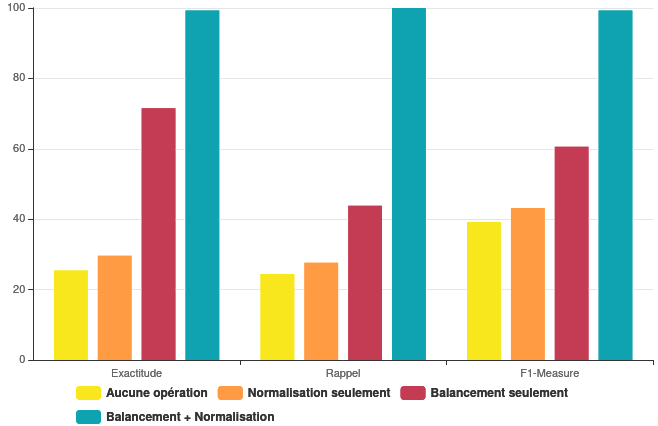
\includegraphics[width=0.95\textwidth]{Figures/performances}
\decoRule
\caption{Comparaison entre les résultats obtenus selon l'opération de prétraitement effectuée}
\label{fig:histogramme}
\end{figure} 
\newpage
En analysant l'histogramme ci-dessus, on voit clairement la différence si applique juste l'opération de normalisation ou l'opération de balancement ou les deux opérations à la fois. On choisisant la bonne méthode de normalisation ainsi 
que celle de balancement, nous avons pu faire passer le taux d'exactitude de notre modèle de \textbf{25.4\%} à \textbf{99.3\%}. Le choix des méthodes était selon une stratégie étudiée et  une synthèse des résultats de plusieurs test effectués sur notre dataset. Les bonnes performances d'un modèle sont toujours engendrées par un bon prétraitement des données.

\newpage
\section{Simulation}
La simulation sera faite à l'aide de Mininet(2.2), qui est installé à coté de Ryu(4.3) sur une machine UBUNTU 20.04 LTS dotée d'un processus i5-6200U et 8Go de RAM. Le réseau qu'on veut simulé contient les élément suivants: un contrôleur SDN, un switch OpenFlow, un serveur de fichiers, un serveur d'applications, 3 hôtes (2 hôtes attaquants at un hôte victime), et essentielement notre système détection F-DoS.
\begin{figure}[h]
\centering
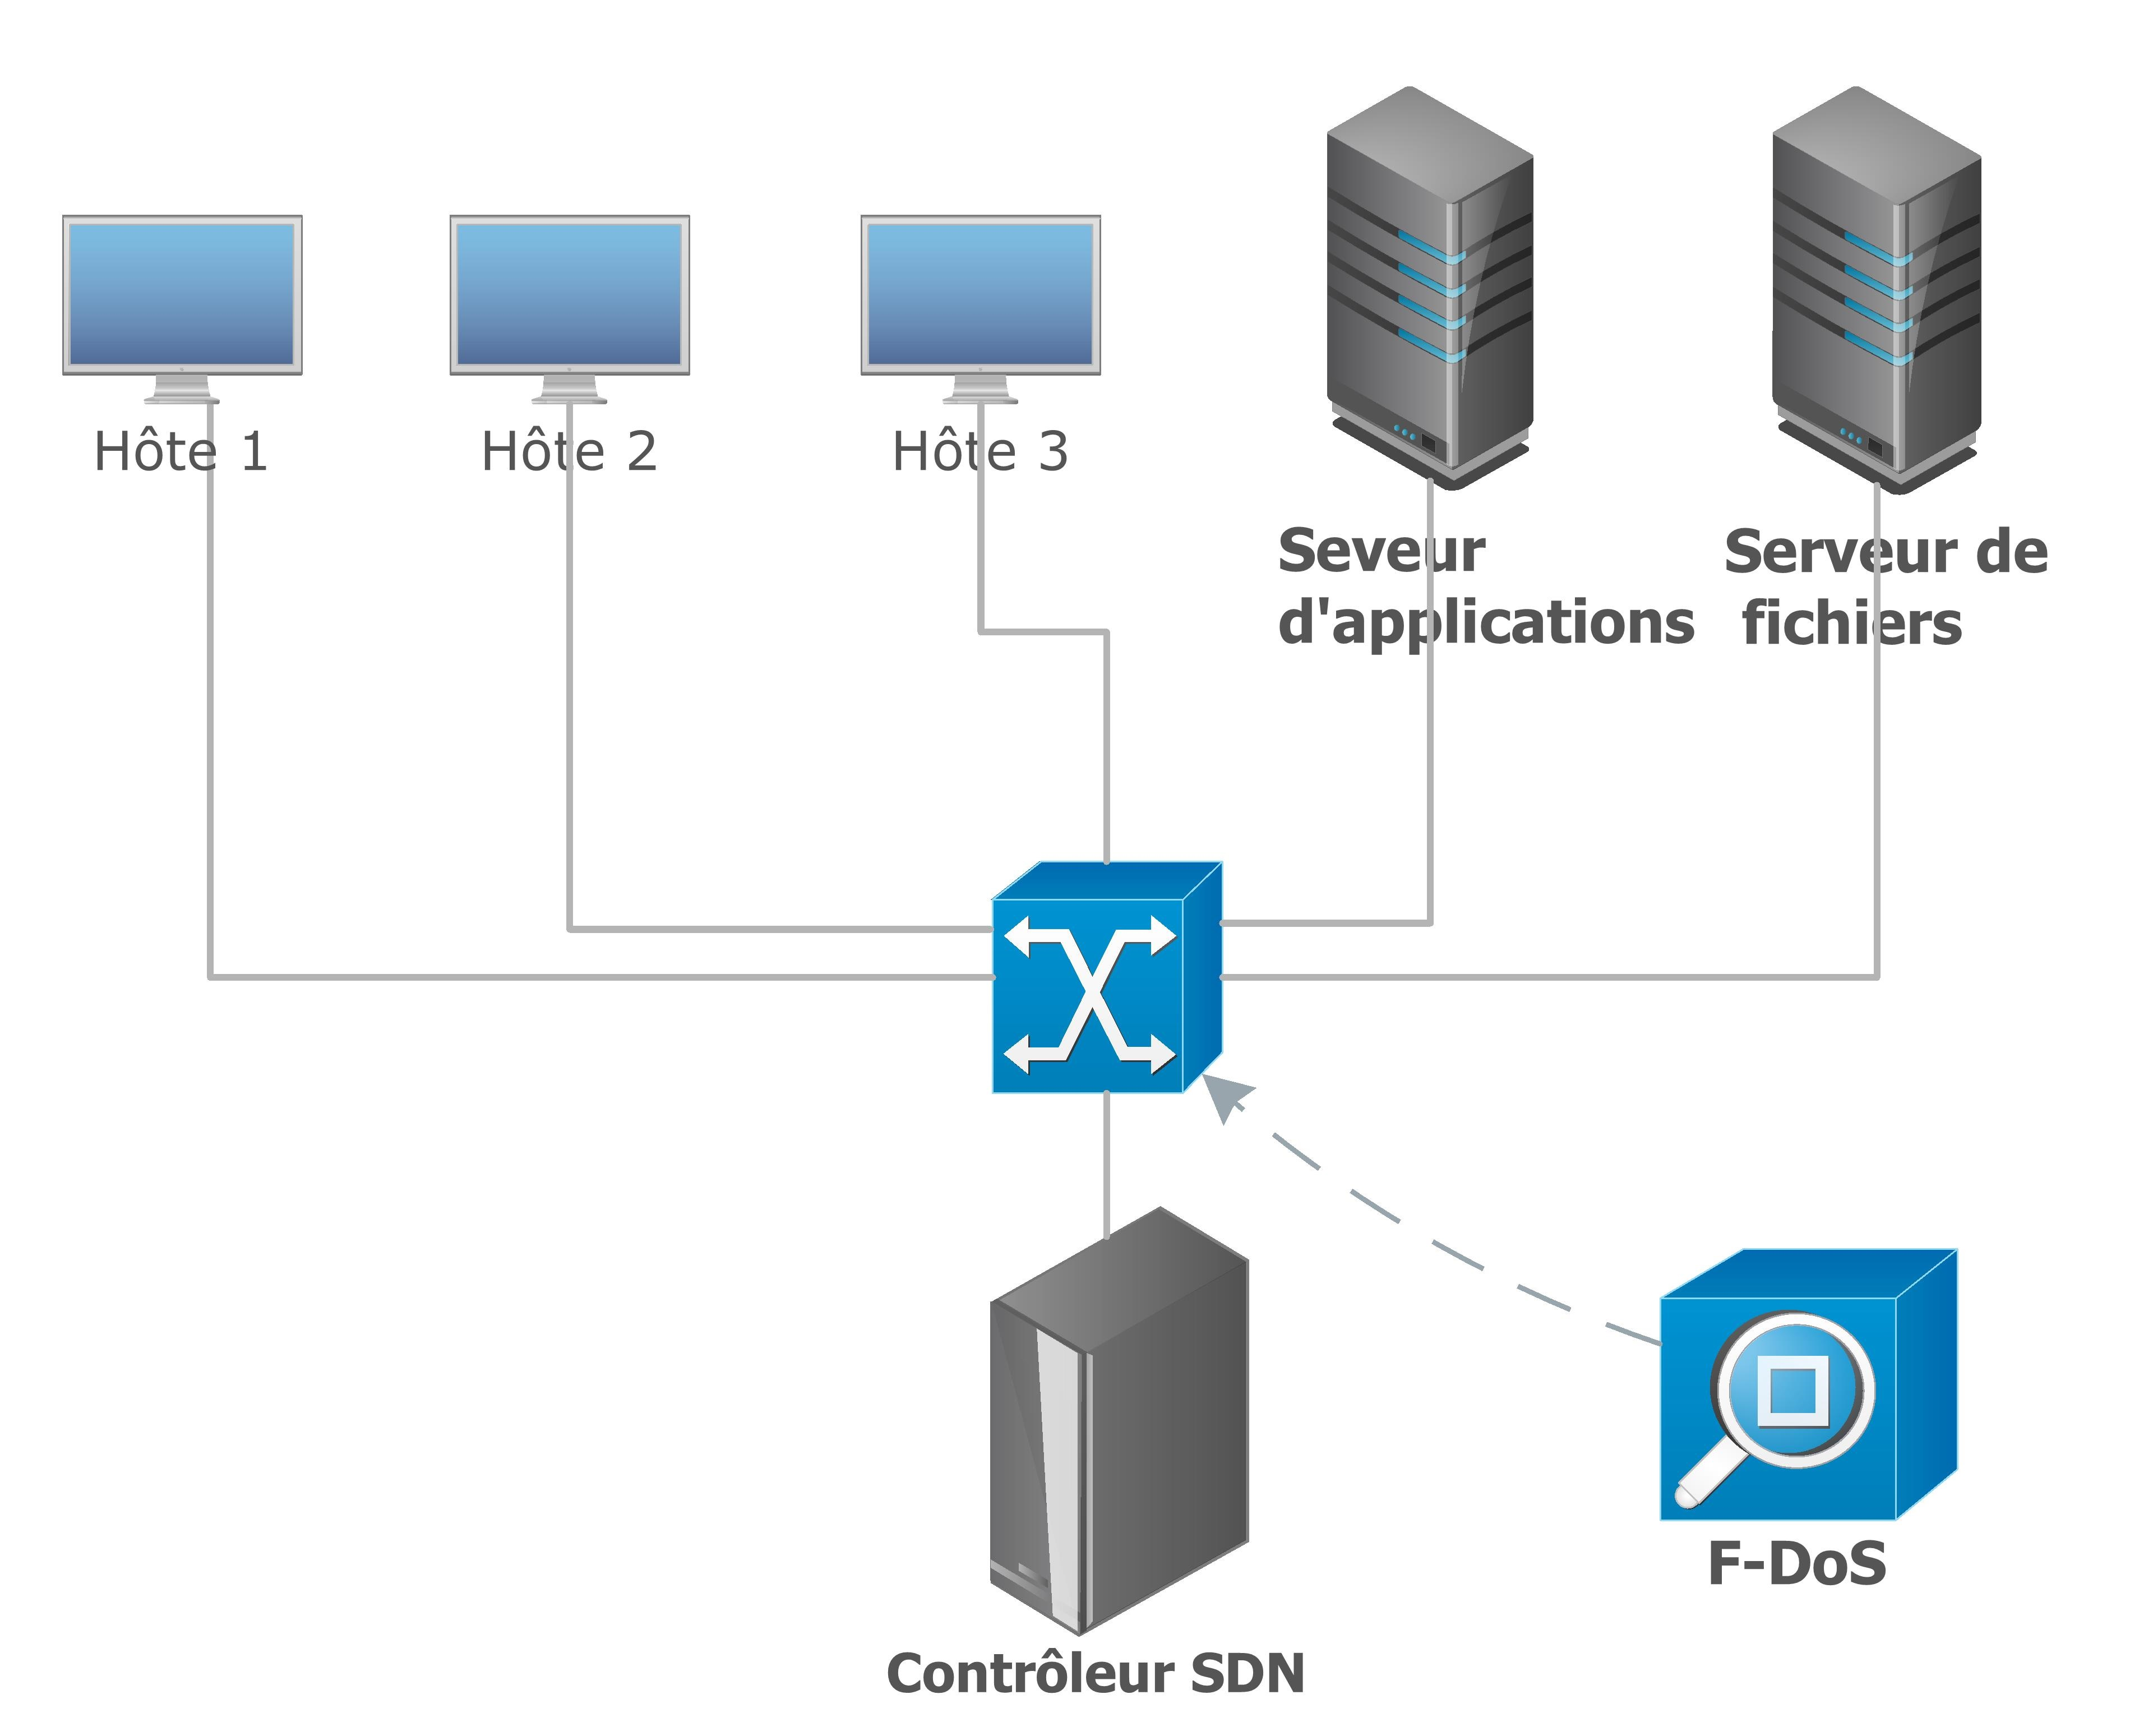
\includegraphics[width=0.8\textwidth]{Figures/simulation}
\decoRule
\caption{Architecture de notre réseau SDN}
\label{fig:architecture}
\end{figure} 

\subsection{Création de la topologie}
Sur mininet nous allons créer la topologie de notre réseau constitué d'un controlleur SDN, un switch OpenFlow, et 6 hôtes qui jouent les rôles illustés dans le tableau \ref{table:nodes}:\\

\noindent Commande de création :
\begin{verbatim}
% sudo mn --controller remote --topo single,6 --switch ovs --mac
\end{verbatim}
Mais faut d'abord lancé le controlleur Ryu avec:
\begin{verbatim}
% ryu-manager ryu_controller.py 
\end{verbatim}

\begin{table}
\begin{center}
\begin{tabular}{  | c || m{5cm} | m{3cm} | }
\hline
\rowcolor[rgb]{0.85,0.85,0.85}
Hôte & Rôle(s) & @IP\\
\hline
\textbf{h6} & Système de détection F-DoS & 10.0.0.6\\
\hline
\textbf{h5} & Serveur d'applications & 10.0.0.5\\
\hline
\textbf{h4} & Serveur de fichiers & 10.0.0.4\\
\hline
\textbf{h3} & hôte victime & 10.0.0.3\\
\hline
\textbf{h2} & Client de \textbf{h5} ou attaquant & 10.0.0.2\\
\hline
\textbf{h1} & Client de \textbf{h4} ou attaquant & 10.0.0.1\\
\hline
\end{tabular}
\caption{Rôle de chaque hôte dans la topologie mininet}
\label{table:nodes}
\end{center}
\end{table}

\begin{figure}[h]
\centering
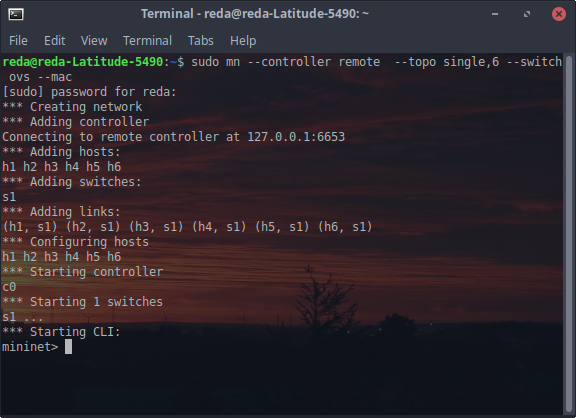
\includegraphics[width=0.7\textwidth]{Figures/simulation/mininet/start}
\decoRule
\caption{Création de la topologie sous mininet}
\label{fig:topologie}
\end{figure}

\newpage
La figure \ref{fig:topologie} indique que la topologie a été créés avec succée et la console mninet est active. On peut voir le contrôleur \textbf{c0}, le switch \textbf{s1} et les différents liens établis (h1, s1), (h2, s1), ..etc. Létape suivante consiste à configurer chaque hôte selon notre topologie.

\subsection{Installation des fonctions}
Jusqu'a présent les hôtes créés par mininet, ainsi que les switch OF, ont les fonctions de base définies par mininet. Donc on doit passer par tous hôte, à l'exeption de h3, pour installer les fonction désignées dans le tableau \ref{table:nodes}. Sur le switch, nous allons juste activer la fonction \textit{Port-Mirroring} comme suit:

\begin{figure}[h]
\centering
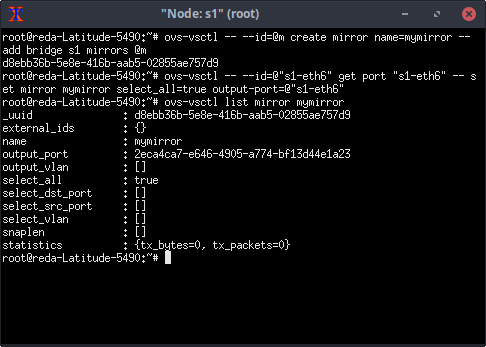
\includegraphics[width=0.7\textwidth]{Figures/simulation/mininet/switch/create_mirroring_port}
\decoRule
\caption{Activation du Port-Mirroring}
\label{fig:topologie}
\end{figure}

\newpage
\subsubsection{A- Installation du système F-DoS sur h6}
Sur l'hôte h6, nous allons installer notre système de détection. Rappelons que le module MEI du système F-DoS est 
Donc en premier nous allons activer le serveur argus sur l'hôte h6 à l'aide de la commande suivante:
\begin{verbatim}
% sudo argus -d -i h6-eth0 -P 561 -w /captured/today.argus
\end{verbatim}
Ensuite on lance le script "IDS.py" qui va installer le client argus, ainsi que le modèle de clustering \textbf{F-Clustering}.
\begin{figure}[h]
\centering
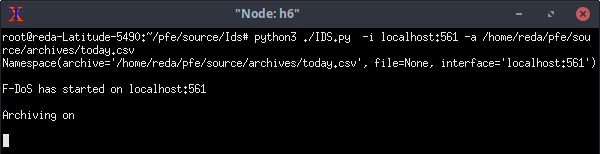
\includegraphics[width=0.9\textwidth]{Figures/simulation/mininet/IDS/start}
\decoRule
\caption{Installation du module de détection}
\label{fig:topologie}
\end{figure}

\subsubsection{B- Installation du seveur d'applications sur h5}
Le fonctionnement de ce serveur est basique, il se met à l'écoute des requêtes des clients, qui sont juste des messages, pour répondre avec un message "hello". Sur l'hôte h5, le script "udpServer.py" est executé comme montré dans la figure \ref{fig:udpServer}.
\begin{figure}[h]
\centering
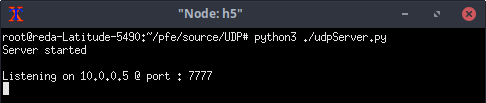
\includegraphics[width=0.9\textwidth]{Figures/simulation/mininet/UDP/server/start}
\decoRule
\caption{Installation du serveur d'applications}
\label{fig:udpServer}
\end{figure}

\subsubsection{B- Installation du seveur de fichier sur h4}
\begin{figure}[h]
\centering
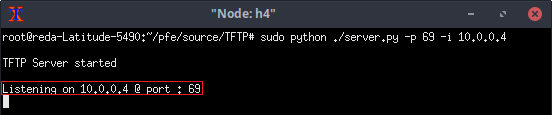
\includegraphics[width=0.9\textwidth]{Figures/simulation/mininet/TFTP/server/start}
\decoRule
\caption{Installation du seveur de fichiers}
\label{fig:udpServer}
\end{figure}